\chapter{Dataset Preparation }
After evaluating the performance of pre-trained models, and with discussions with other subgroups, it became evident that training on a custom dataset tailored to our specific requirements was necessary. Consequently, we curated a dataset comprising images of boxes, which served as the foundation for training our image segmentation model.

\section{Roboflow Implementation Trials 10/3/2024}
We discovered a platform called Roboflow (\url{https://roboflow.com/}) that offers pre-trained datasets, streamlining the process of dataset preparation and integration. We leveraged one of their datasets specifically tailored for image segmentation tasks, comprising 333 images for training, 94 images for validation, and 48 images for testing. This particular dataset had been successfully utilized by other Roboflow users, yielding promising segmentation results, further reinforcing our decision to adopt it for our project.

\begin{figure}[H]
      \centering
      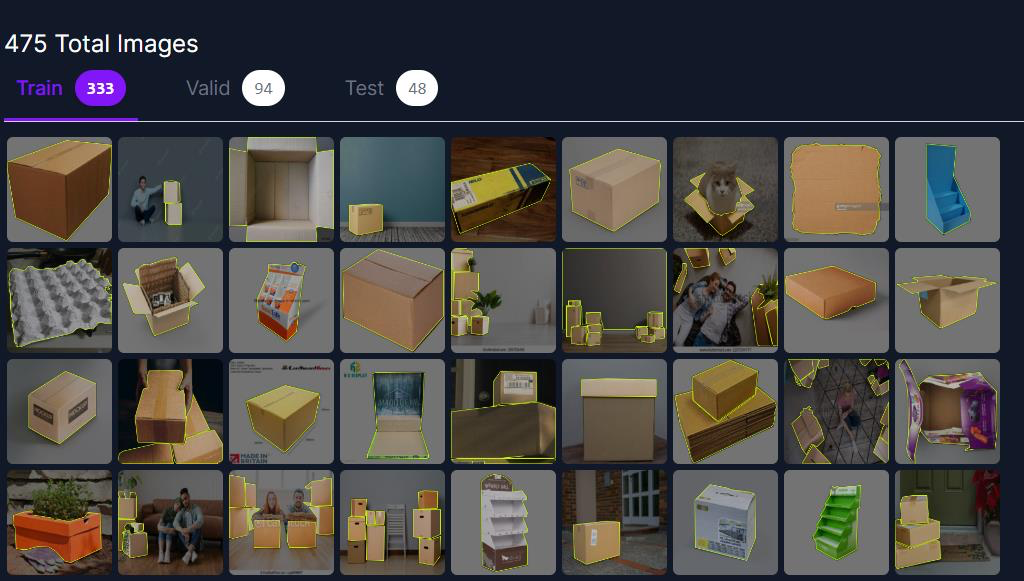
\includegraphics[width=450pt]{assets/roboflow}
      \caption{Roboflow Dataset Generation in Their Website}
      \label{fig:using:roboflowgen}
\end{figure}

Another reason why Roboflow was selected is it’s builtin interfaces for deploying in a Google Colab environment using a simple API call.

Here is how to port a Roboflow dataset in Google Colab:
\begin{lstlisting}[language=Python]
# 1.install the roboflow package
!pip install roboflow

# 2.dataset can be called
from roboflow import Roboflow
rf = Roboflow(api_key="########")
project = rf.workspace("vnudc").project("cardboard-boxes-vnal0")
version = project.version(1)
dataset = version.download("tensorflow")

# 3.use the dataset with your model
...
\end{lstlisting}

But when using this dataset to feed to the SegNet model we cam across this issue.

\begin{lstlisting}[language=bash]
TypeError: join() argument must be str, bytes, or os.PathLike object, 
not 'int'
\end{lstlisting}

We found out that this error is due to a mismatch of the format of the ported dataset with the format required by the model to split the dataset in to train , test and validate sets. We have to look into solve this error later.

\section{Self Curated Dataset 20/3/2024}
The dataset preparation phase is a critical component of the image segmentation pipeline, as the quality and diversity of the training data significantly influence the model's performance and generalization capabilities. In this regard, our expectations for the curated dataset encompass the following key aspects:

\subsection{Expectations}
\begin{description}
      \item[Representativeness]
            The dataset should be representative of the industrial scenarios and applications for which the image segmentation model is intended. It should capture a diverse range of object shapes, sizes, orientations, and backgrounds to ensure the model's robustness and ability to generalize effectively. This was achieved by hand picking the source images and using advanced ImageGen tools to generate variations of settings to speed up the collection process.

      \item[Annotation Quality]
            Accurate and consistent annotations are essential for training accurate segmentation models. The dataset should be meticulously annotated, with precise delineation of object boundaries and correct labeling of object classes. Since leveraging semi-automated annotation tools can contribute to maintaining high annotation quality, it was proposed as a viable method in a discussion. This was further expanded later to review many annotation tools in the web which are open-source.

      \item[Scalability]
            As the project progresses, the dataset should be easily scalable to accommodate additional data and annotations. This scalability will enable us to iteratively expand the dataset, thereby improving the model's performance and addressing potential biases or limitations identified during the training and evaluation phases. Review of literature material to achieve this is still undergoing.

      \item[Multi-model Compatibility]
            To facilitate comprehensive testing and bench-marking, the dataset should be compatible with multiple state-of-the-art image segmentation models and architectures. This compatibility will allow for comparative analyses and informed decision-making when selecting the most suitable model for our specific use case. With the initial discussion our subgroup decided to replicate the same features of the CamVid dataset, and then cross referencing with other subgroups lead to further literary review. Further Review to achieve this is still undergoing.

      \item[Common Mistake Mitigation]
            During the dataset creation process, it is essential to account for and mitigate common mistakes that can undermine the model's performance. These mistakes may include:
\end{description}

\begin{description}
      \item[Class Imbalance:] Ensuring a balanced distribution of object classes within the dataset is crucial to prevent the model from being biased toward dominant classes. This is achieved by simplifying the classes we wanted in our model to a lower number and focusing on finding the box first around the center. This might introduce some problems with navigation of the arm when cargo is uniquely positioned. Further review required.
      \item[Annotation Inconsistencies] Establishing clear annotation guidelines and conducting regular quality checks can help maintain consistency in the annotations across the dataset. All our subgroups decided to implement annotation as masks as it would allow for greater detail for certain models and can be simplified to a polygon if required later.
      \item[Data Leakage:] Proper dataset splitting and separation of training, validation, and test sets are necessary to prevent data leakage, which can lead to overly optimistic performance evaluations. We are tracking this problem in our goals, but since this is a problem that raises with scale and we are currently targeting a smaller database we decided to postpone this.
\end{description}

By addressing these expectations and proactively mitigating potential pitfalls, we aim to create a robust and versatile dataset that can serve as a solid foundation for training and evaluating our image segmentation models, ultimately contributing to the development of an efficient and accurate segmentation system.

\subsection{Implementation Trail}
This dataset comprised annotated images depicting various types of boxes commonly encountered in bin picking scenarios. Annotating these images with bounding box coordinates facilitated the training of our object detection models, ensuring they could accurately localize and classify boxes in real-world environments.

Many alternatives were looked upon and plans were made about the exact implementation of dataset with several brainstorming sessions within the subgroup and among the subgroups.

\begin{figure}[h]
      \centering
      \begin{subfigure}[b]{0.45\textwidth}
            \centering
            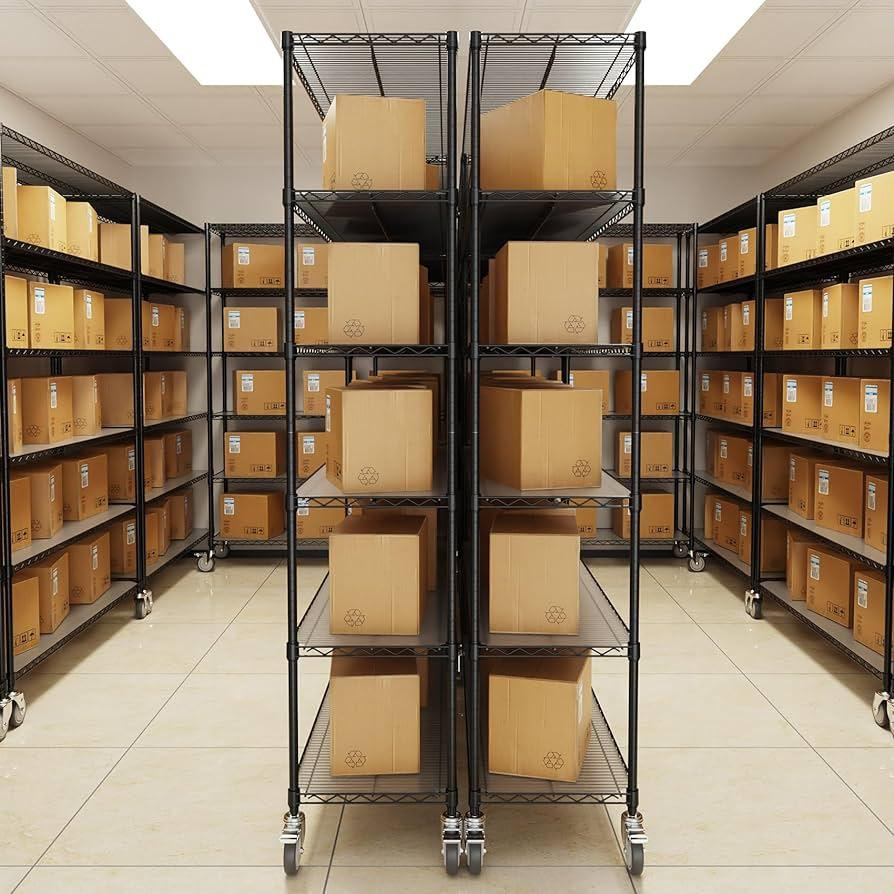
\includegraphics[width=\textwidth]{assets/dataset/img.jpeg}
            \caption{Sample image from our custom dataset}
      \end{subfigure}
      \hfill
      \begin{subfigure}[b]{0.45\textwidth}
            \centering
            
\includegraphics[width=\textwidth]{assets/dataset/mask.jpeg}
            \caption{Corresponding mask for the image}
      \end{subfigure}
      \caption{Sample image pair from the custom dataset}
\end{figure}

\begin{figure}[h]
      \centering
      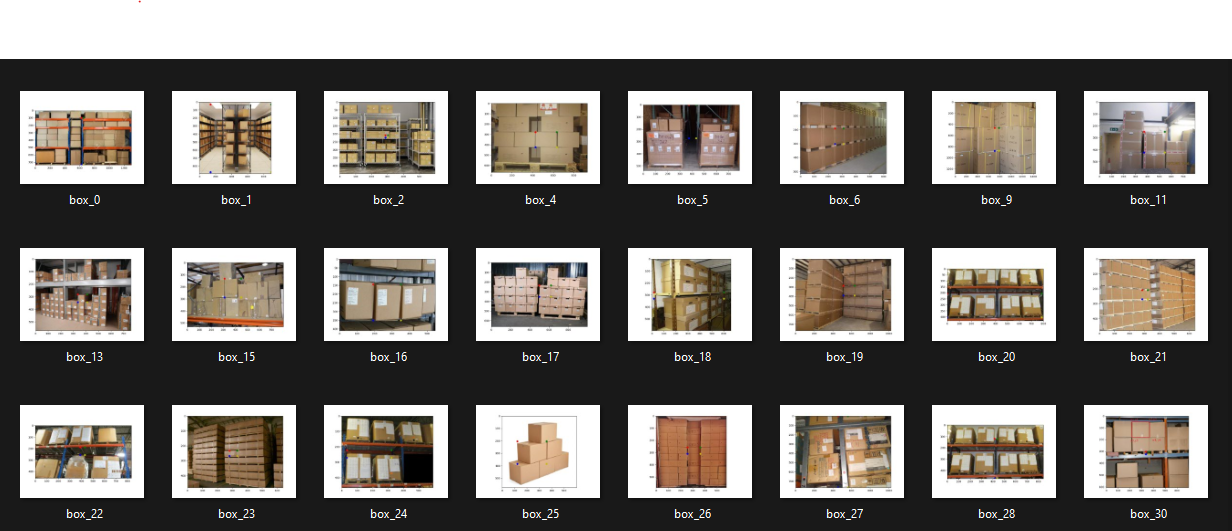
\includegraphics[width=14cm]{assets/dataset/original_dataset.png}
      \caption{Snapshot of original images in our custom dataset}
\end{figure}

\begin{figure}[h]
      \centering
      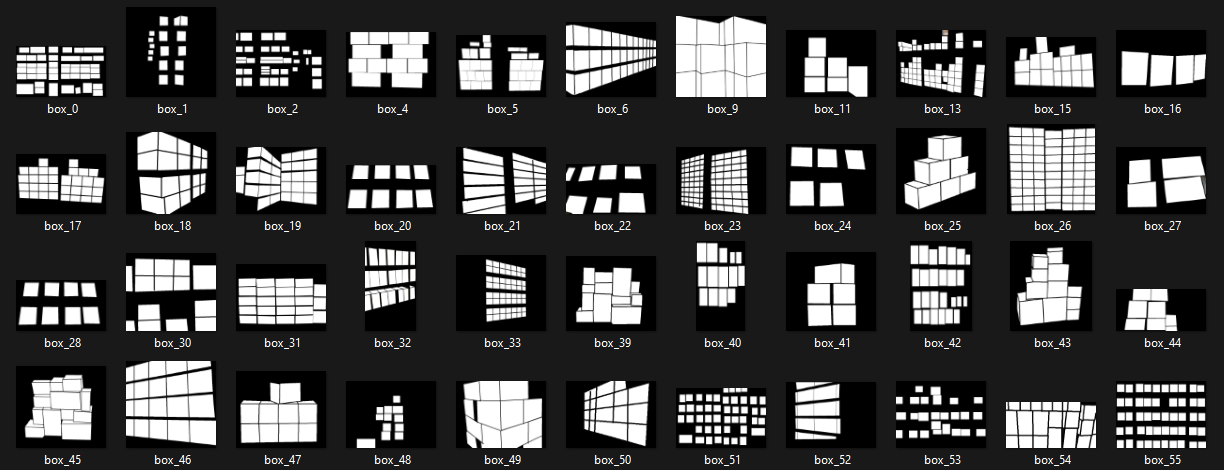
\includegraphics[width=14cm]{assets/dataset/annotated_dataset.png}
      \caption{Snapshot of annotated images in our custom dataset}
\end{figure}